\subsection{SV required strategies}

\subsubsection{GW gold}

% - Epochs now handled properly

\begin{table}
\centering
\begin{adjustbox}{max width=\textwidth}
\begin{tabular}{|l|l|l|l|l|l|l|l|}
\hline
Expected night & Resulting night & Expected visits & Resulting visits & Expected filters & Resulting filters & Expected exposure times & Resulting exposure times \\ \hline
0              & 0               & 3               & 3                & gri              & gri               & 120                     & 120                      \\ \hline
1              & 1               & 1               & 1                & gi               & gi                & 180                     & 180                      \\ \hline
2              & 2               & 1               & 1                & gi               & gi                & 180                     & 180                      \\ \hline
3              & 3               & 1               & 1                & gi               & gi                & 180                     & 180                      \\ \hline
\end{tabular}
\end{adjustbox}
\caption{Results of the GW: NS gold ToO testing}
\label{tab:GWGoldResults}
\end{table}

\begin{figure}
    \centering
    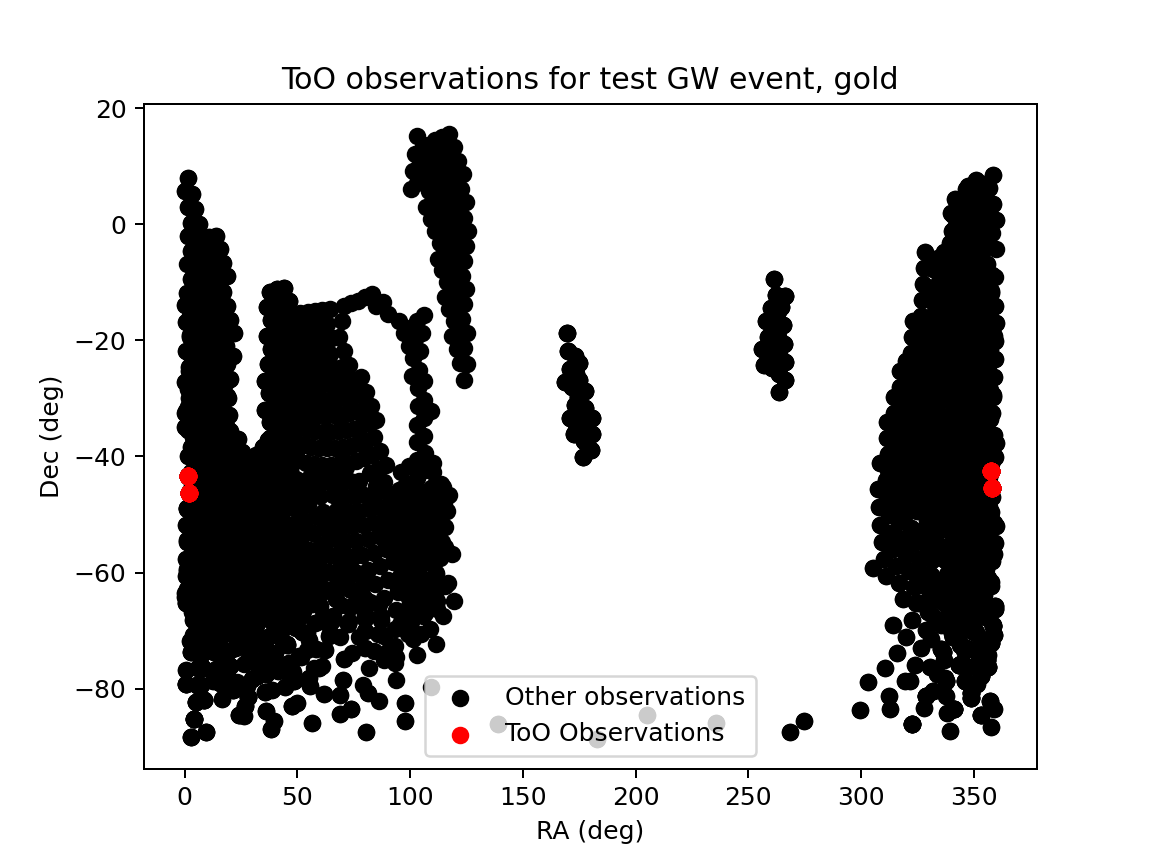
\includegraphics[width=\linewidth]{figures/validationTests/SVRequired/GWGoldPosition.png}
    \caption{Results from GW: NS Gold ToO visits over a 5 day LSST simulation}
    \label{fig:GWGoldPositionResult}
\end{figure}

\begin{figure}
    \centering
    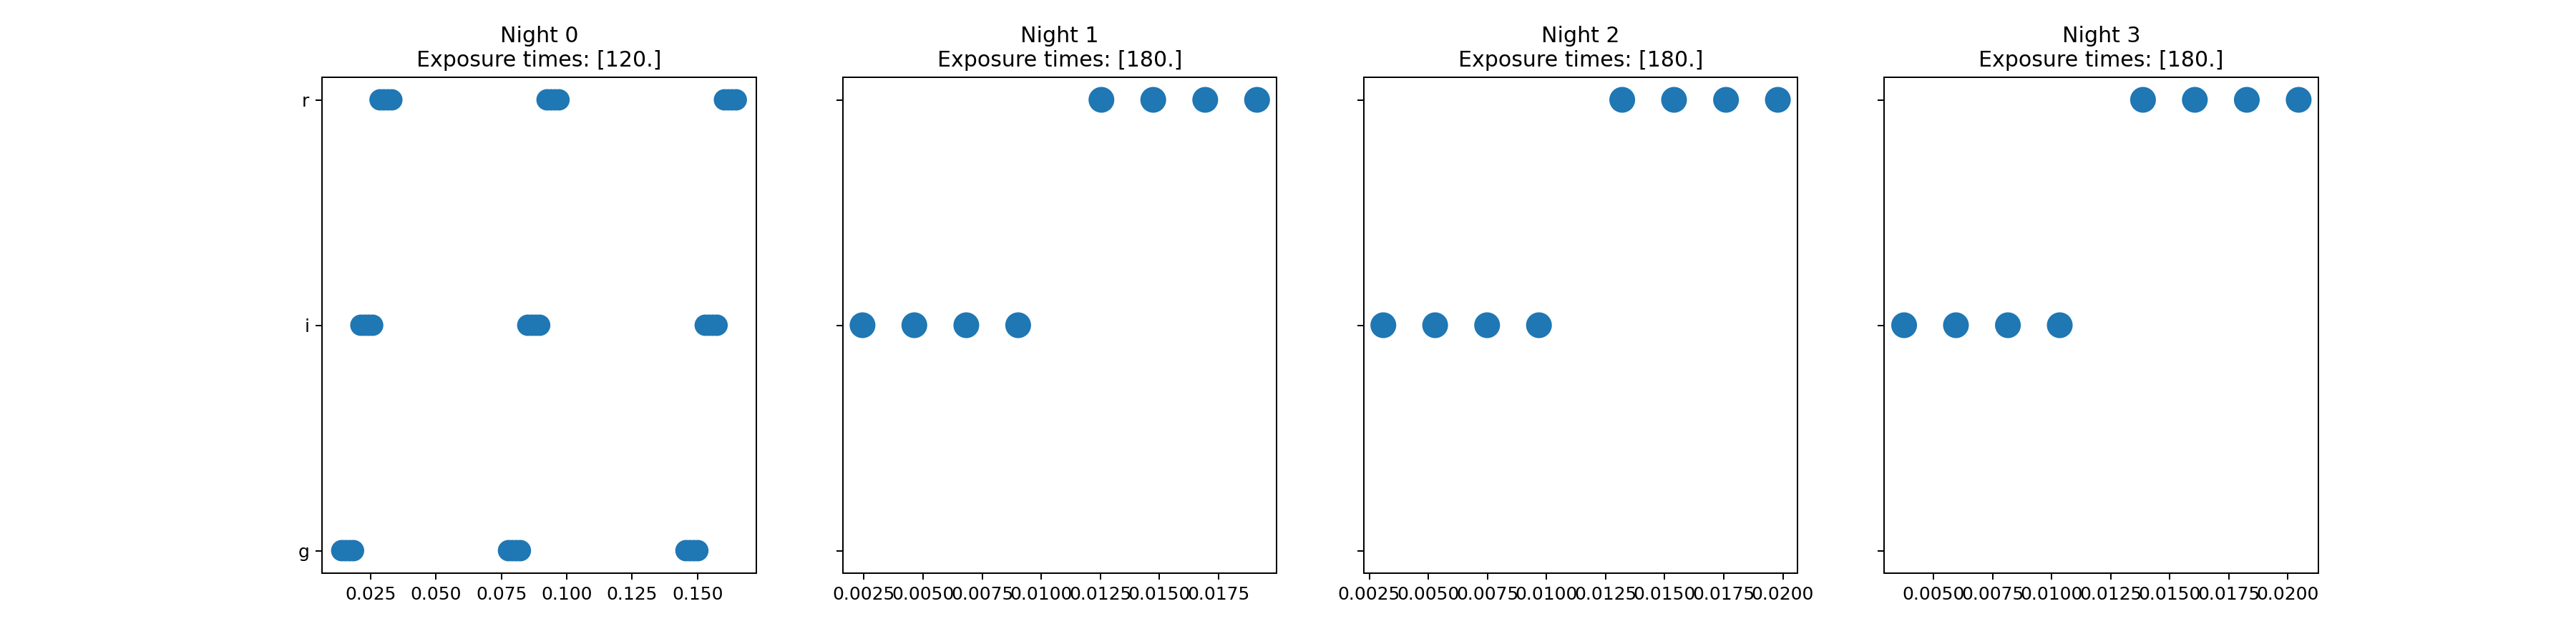
\includegraphics[width=\linewidth]{figures/validationTests/SVRequired/GWGoldFilterPlot.png}
    \caption{Results from GW: NS Gold ToO filter and visit distribution over a 5 day LSST simulation}
    \label{fig:GWGoldFilterResult}
\end{figure}

\newpage

\subsubsection{GW Silver}

\begin{table}[h]
\centering
\begin{adjustbox}{max width=\textwidth}
\begin{tabular}{|l|l|l|l|l|l|l|l|}
\hline
Expected night & Resulting night & Expected visits & Resulting visits & Expected filters & Resulting filters & Expected exposure times & Resulting exposure times \\ \hline
0              & 0               & 1               & 1                & gi               & gi                & 30                      & 30                       \\ \hline
1              & 1               & 1               & 1                & gi               & gi                & 120                     & 120                      \\ \hline
2              & 2               & 1               & 1                & gi               & gi                & 120                     & 120                      \\ \hline
3              & 3               & 1               & 1                & gi               & gi                & 120                     & 120                      \\ \hline
\end{tabular}
\end{adjustbox}
\caption{Results of the GW: NS silver ToO testing}
\label{tab:GWSilverResults}
\end{table}

\begin{figure}
    \centering
    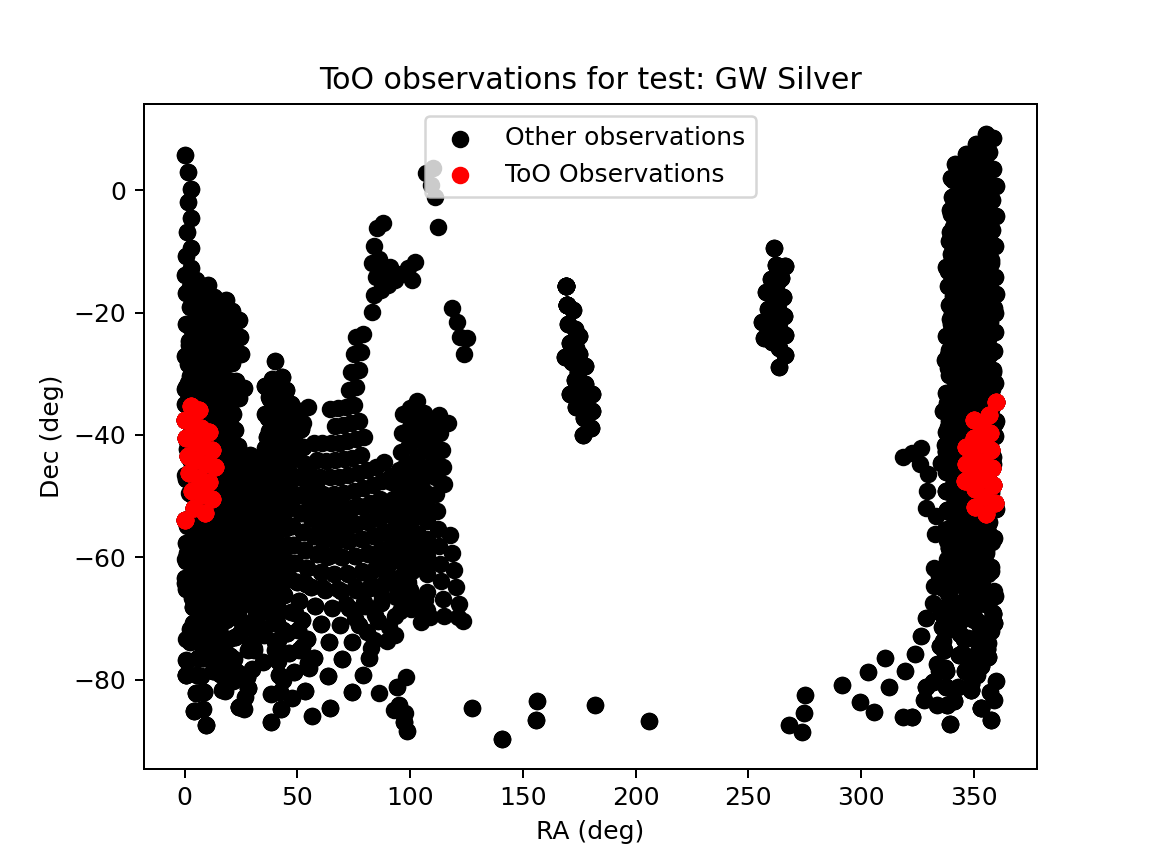
\includegraphics[width=\linewidth]{figures/validationTests/SVRequired/GWSilverPosition.png}
    \caption{Results from GW: NS Silver ToO visits over a 5 day LSST simulation}
    \label{fig:GWSilverPositionResult}
\end{figure}

\begin{figure}
    \centering
    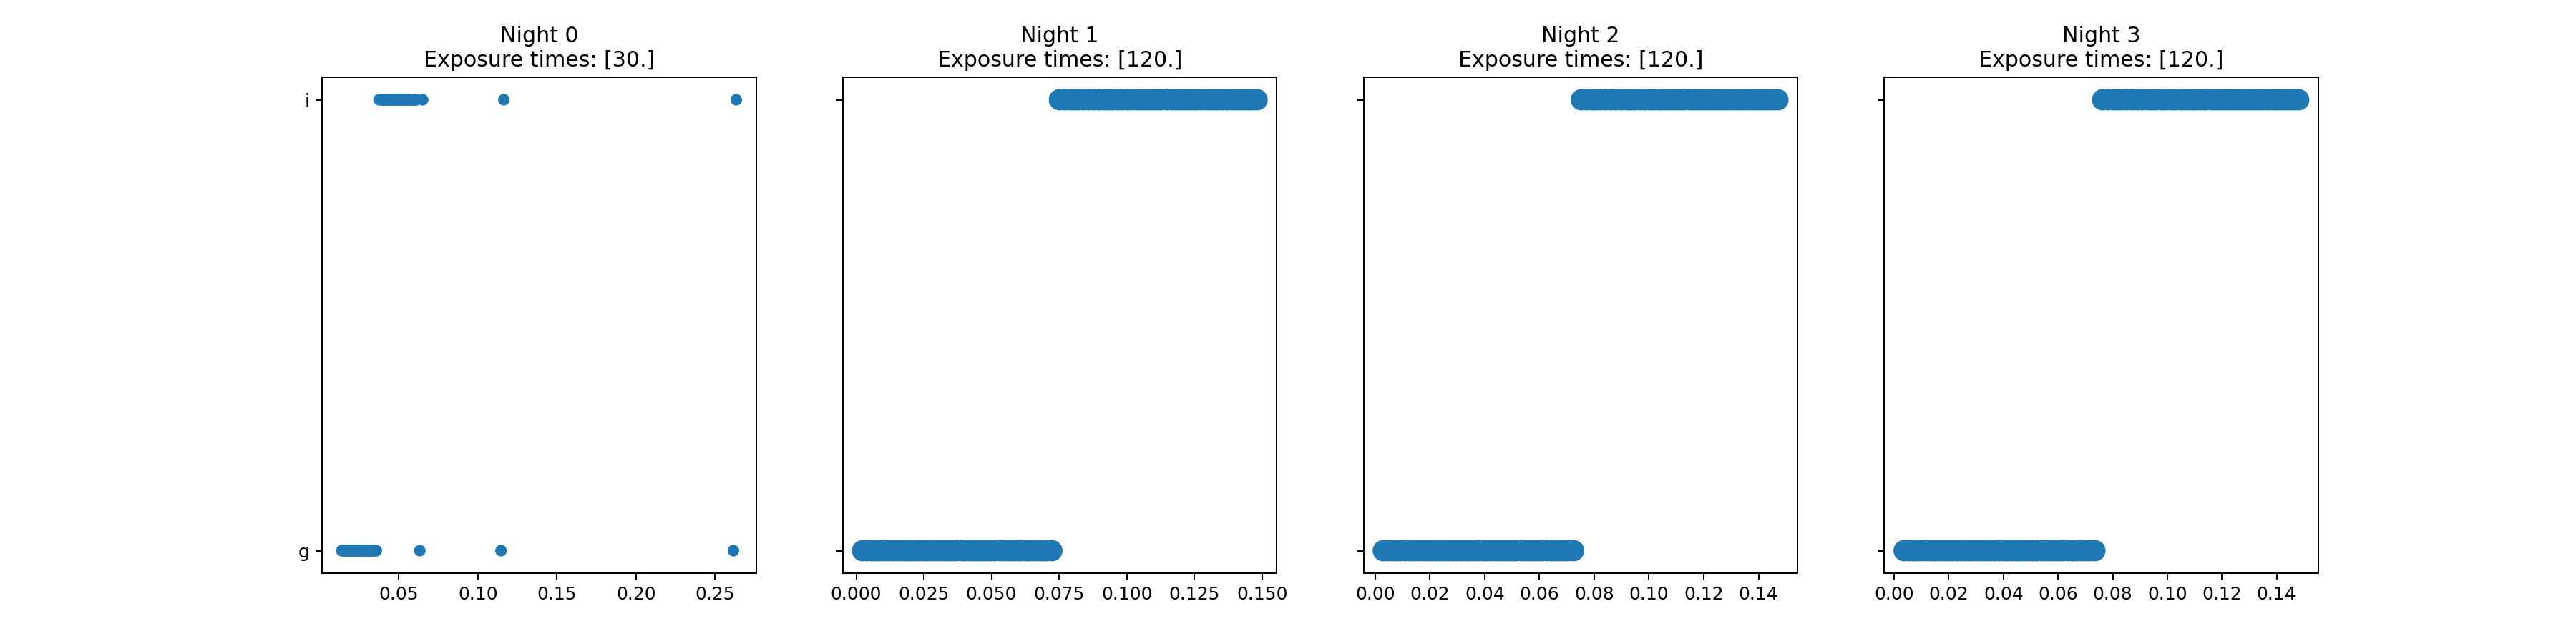
\includegraphics[width=\linewidth]{figures/validationTests/SVRequired/GWSilverFilterPlot.png}
    \caption{Results from GW: NS Silver ToO filter and visit distribution over a 5 day LSST simulation}
    \label{fig:GWSilverFilterResult}
\end{figure}
\newpage
\subsubsection{GW BBH}

\paragraph{Dark time, distant event}

\begin{table}[h]
\centering
\begin{adjustbox}{max width=\textwidth}
\begin{tabular}{|l|l|l|l|l|l|l|l|}
\hline
Expected night & Resulting night & Expected visits & Resulting visits & Expected filters & Resulting filters & Expected exposure times & Resulting exposure times \\ \hline
0              & 0               & 1               & 1                & gri              & gri               & 30                      & 30                       \\ \hline
2              & 2               & 1               & 1                & gri              & gri               & 30                      & 30                       \\ \hline
7              & 7               & 1               & 1                & gri              & gri               & 30                      & 30                       \\ \hline
9              & 9               & 1               & 1                & gri              & gri               & 30                      & 30                       \\ \hline
39             & 39              & 1               & 1                & gri              & gri               & 30                      & 30                       \\ \hline
\end{tabular}
\end{adjustbox}
\caption{Results of the GW: BBH, dark time, distant event ToO testing}
\label{tab:GWBBHDarkFarResults}
\end{table}

\begin{figure}
    \centering
    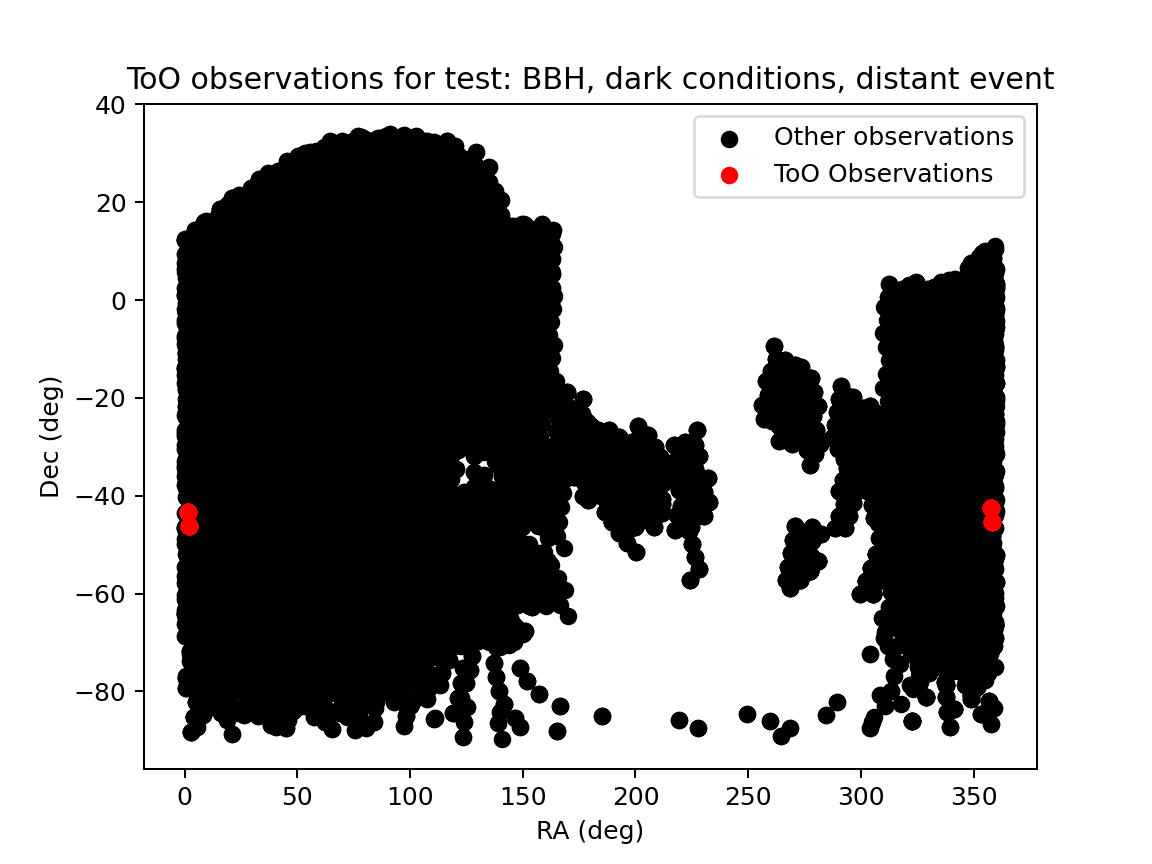
\includegraphics[width=\linewidth]{figures/validationTests/SVRequired/BBHDarkFarPosition.png}
    \caption{Results from GW: BBH, dark conditions, distant event ToO visits over a 5 day LSST simulation}
    \label{fig:GWBBHDarkFarPositionResult}
\end{figure}

\begin{figure}
    \centering
    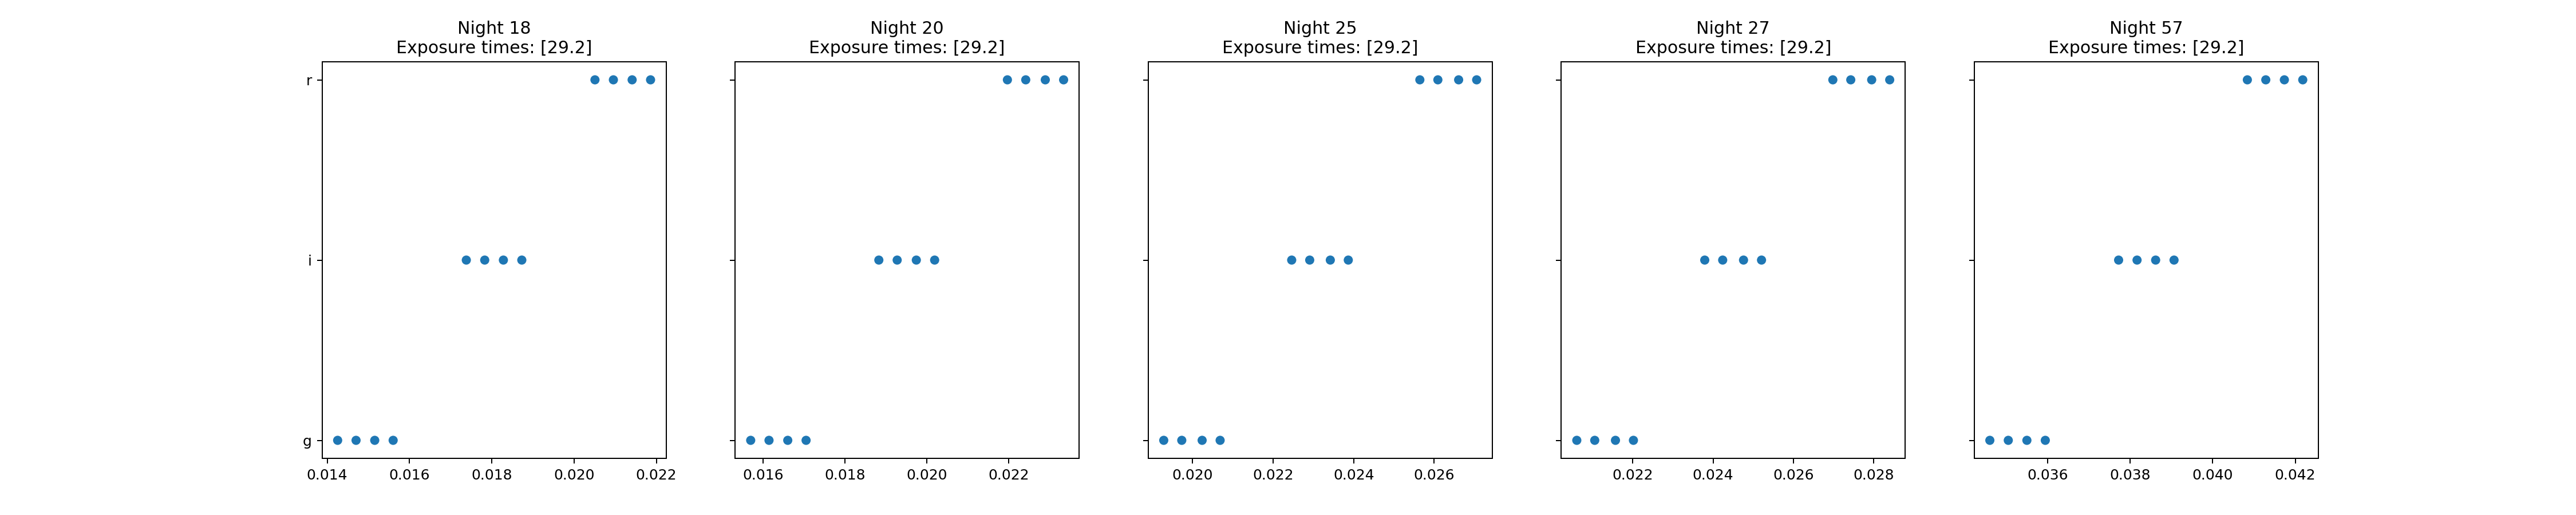
\includegraphics[width=\linewidth]{figures/validationTests/SVRequired/BBHDarkFarFilterPlot.png}
    \caption{Results from GW: BBH, dark conditions, distant event ToO filter and visit distribution over a 5 day LSST simulation}
    \label{fig:GWBBHDarkFarFilterResult}
\end{figure}
\newpage
\paragraph{Dark time, nearby event}

\begin{table}[]
\centering
\begin{adjustbox}{max width=\textwidth}
\begin{tabular}{|l|l|l|l|l|l|l|l|}
\hline
Expected night & Resulting night & Expected visits & Resulting visits & Expected filters & Resulting filters & Expected exposure times & Resulting exposure times \\ \hline
0              & 0               & 1               & 1                & ugi              & ugi               & 30                      & 30                       \\ \hline
2              & 2               & 1               & 1                & ugi              & ugi               & 30                      & 30                       \\ \hline
7              & 7               & 1               & 1                & ugi              & ugi               & 30                      & 30                       \\ \hline
9              & 9               & 1               & 1                & ugi              & ugi               & 30                      & 30                       \\ \hline
39             & 39              & 1               & 1                & ugi              & ugi               & 30                      & 30                       \\ \hline
\end{tabular}
\end{adjustbox}
\caption{Results of the GW: BBH, dark time, nearby event ToO testing}
\label{tab:GWBBHDarkNearResults}
\end{table}

\begin{figure}
    \centering
    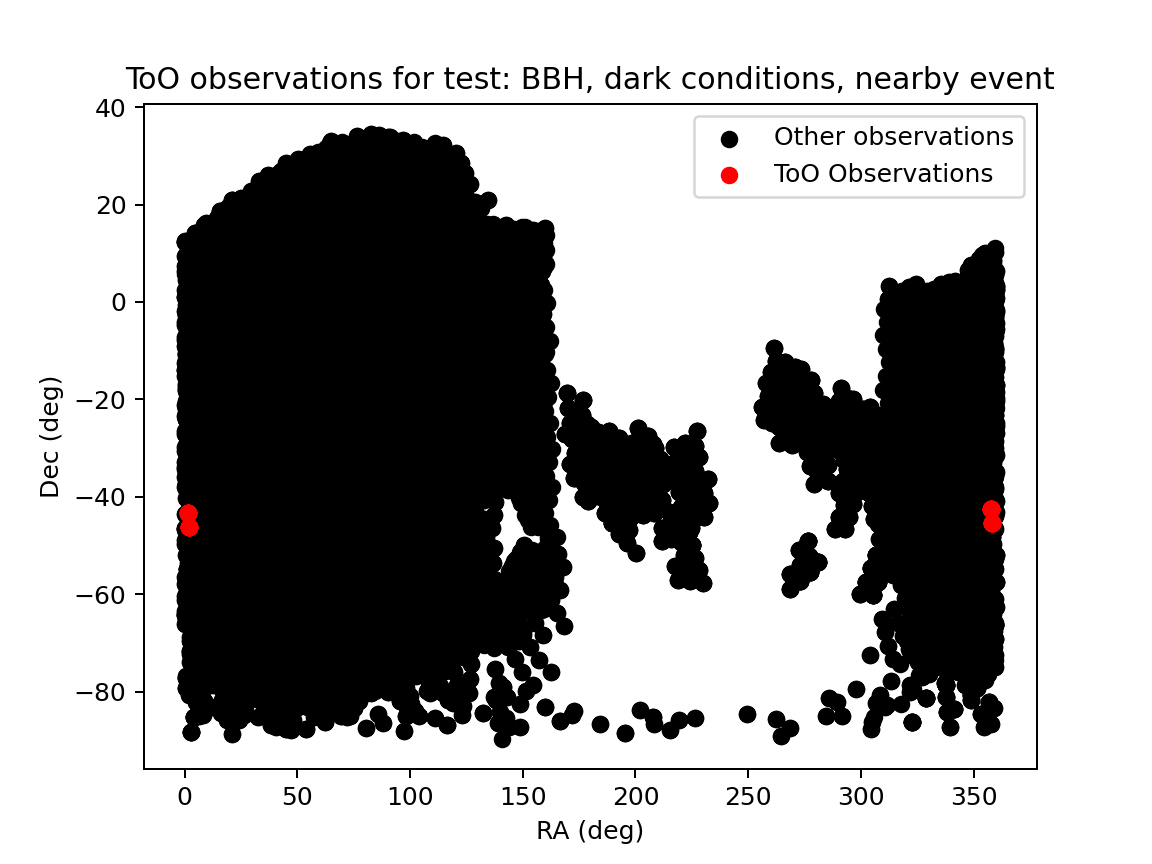
\includegraphics[width=\linewidth]{figures/validationTests/SVRequired/BBHDarkNearPosition.png}
    \caption{Results from GW: BBH, dark conditions, nearby event ToO visits over a 45 day LSST simulation}
    \label{fig:GWDarkNearPositionResult}
\end{figure}

\begin{figure}
    \centering
    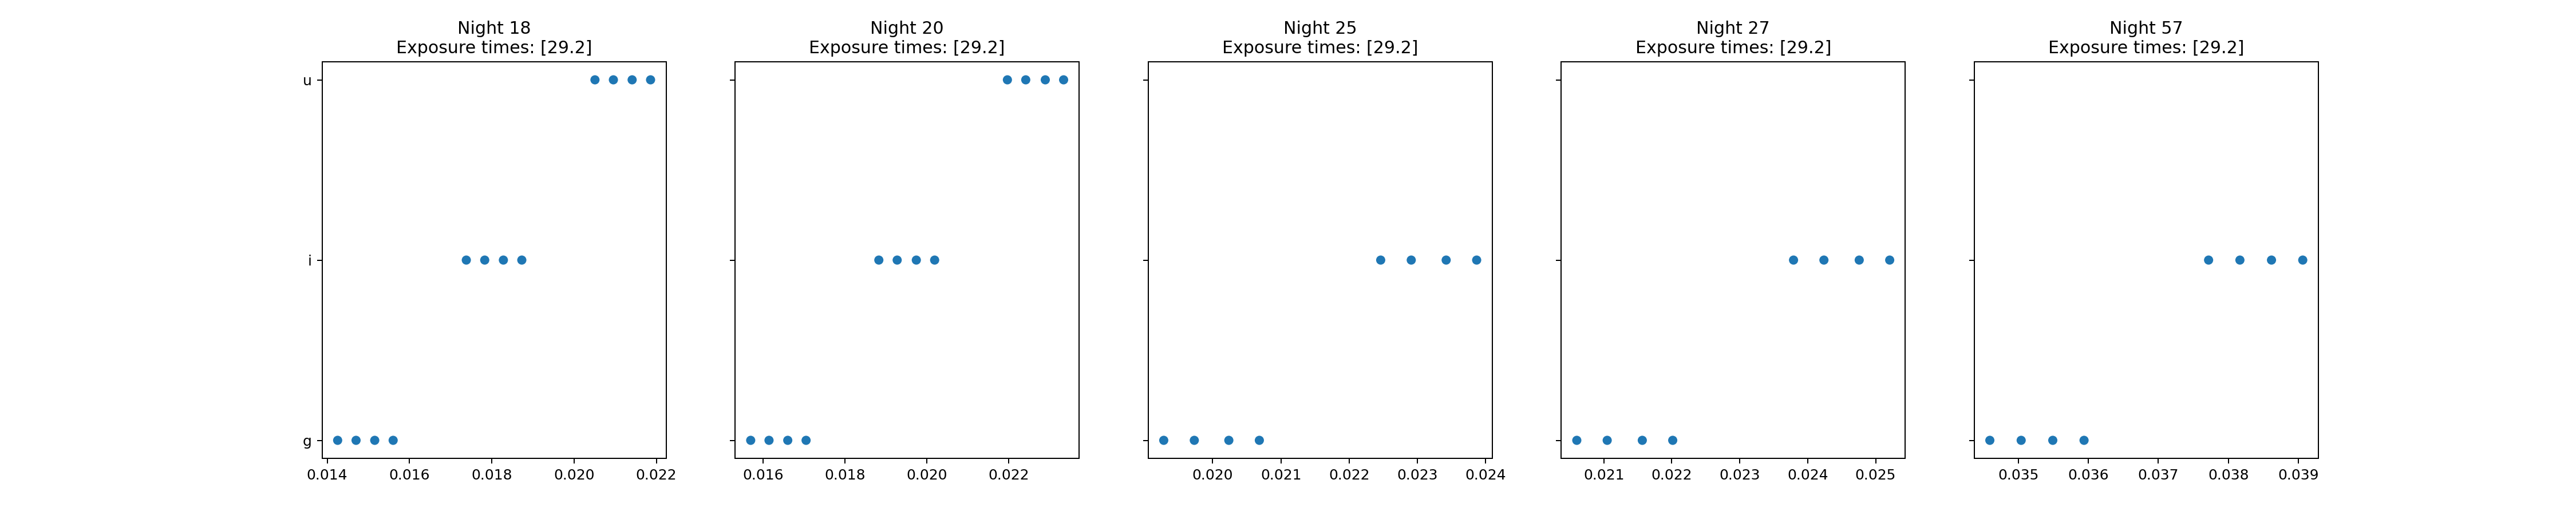
\includegraphics[width=\linewidth]{figures/validationTests/SVRequired/BBHDarkNearFilterPlot.png}
    \caption{Results from GW: BBH, dark conditions, nearby event ToO filter and visit distribution over a 45 day LSST simulation}
    \label{fig:GWDarkNearFilterResult}
\end{figure}
\newpage
\paragraph{Bright time}

\begin{table}[]
\centering
\begin{adjustbox}{max width=\textwidth}
\begin{tabular}{|l|l|l|l|l|l|l|l|}
\hline
Expected night & Resulting night & Expected visits & Resulting visits & Expected filters & Resulting filters & Expected exposure times & Resulting exposure times \\ \hline
0              & 0               & 1               & 1                & riz              & riz               & 30                      & 30                       \\ \hline
2              & 2               & 1               & 1                & riz              & riz               & 30                      & 30                       \\ \hline
7              & 7               & 1               & 1                & riz              & riz               & 30                      & 30                       \\ \hline
9              & 9               & 1               & 1                & riz              & riz               & 30                      & 30                       \\ \hline
39             & 39              & 1               & 1                & riz              & riz               & 30                      & 30                       \\ \hline
\end{tabular}
\end{adjustbox}
\caption{Results from GW: BBH, bright conditions ToO filter and visit distribution over a 45 day LSST simulation}
\label{tab:BBHBrightResults}
\end{table}


\begin{figure}
    \centering
    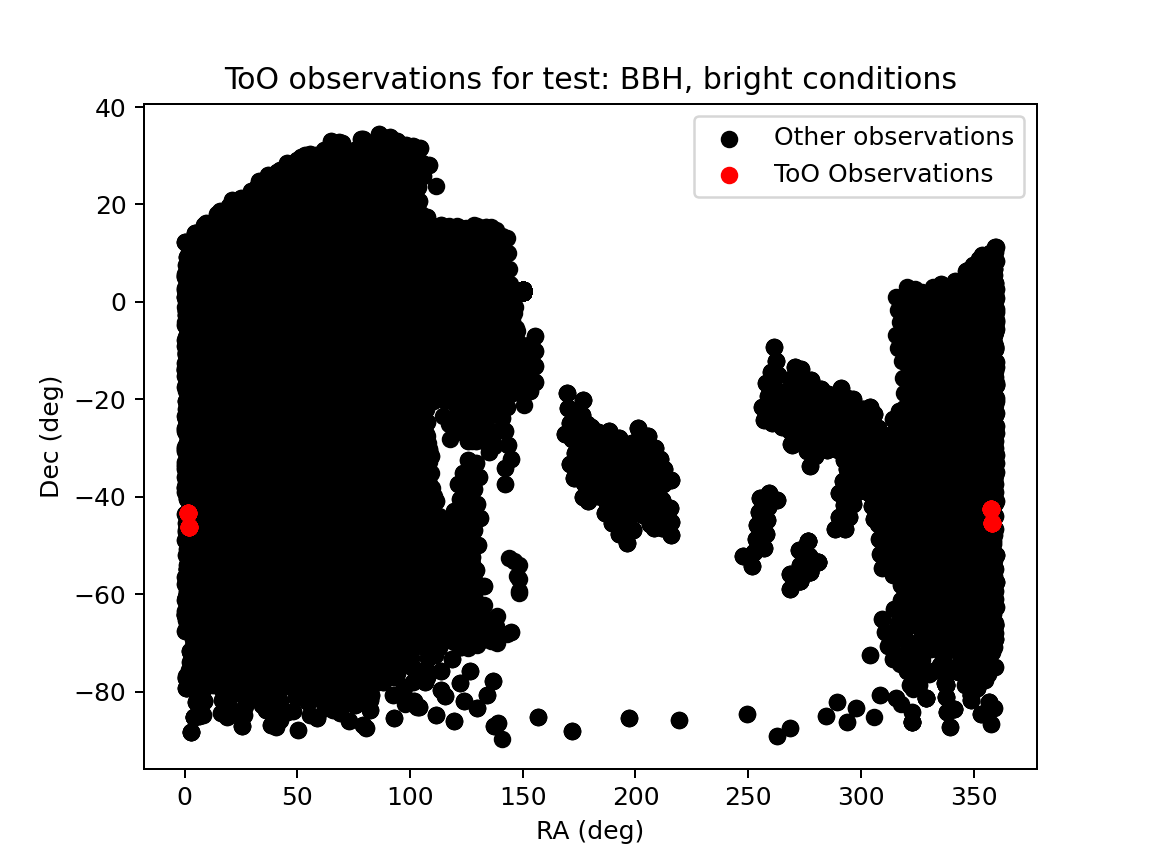
\includegraphics[width=\linewidth]{figures/validationTests/SVRequired/BBHBrightPosition.png}
    \caption{Results from GW: BBH, dark conditions, nearby event ToO visits over a 45 day LSST simulation}
    \label{fig:GWBrightPositionResult}
\end{figure}

\begin{figure}
    \centering
    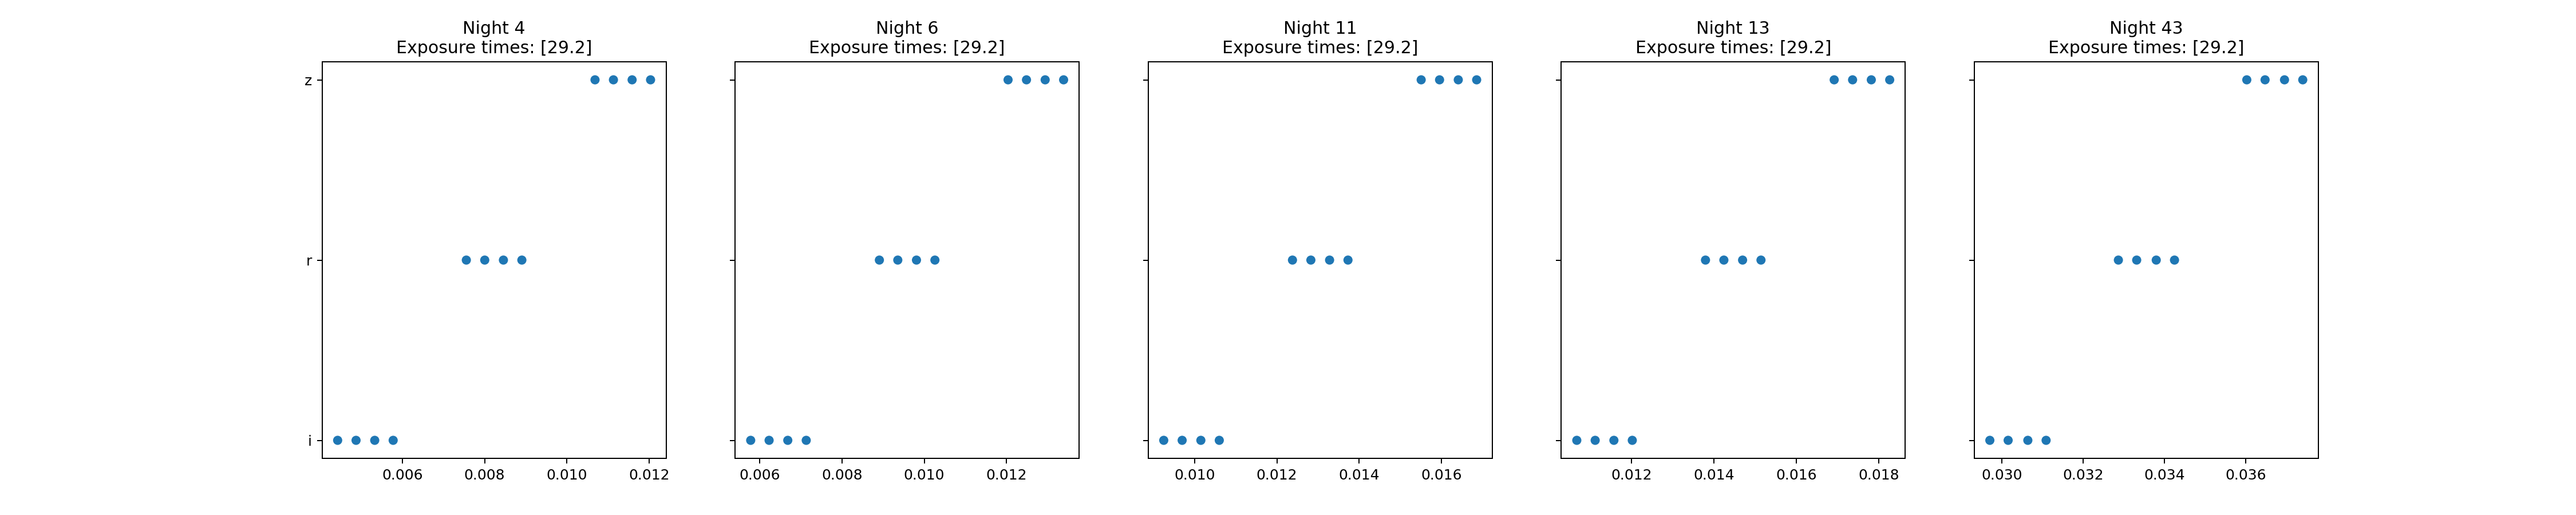
\includegraphics[width=\linewidth]{figures/validationTests/SVRequired/BBHBrightFilterPlot.png}
    \caption{Results from GW: BBH, dark conditions, nearby event ToO filter and visit distribution over a 45 day LSST simulation}
    \label{fig:GWBrightFilterResult}
\end{figure}
\newpage

\subsection{High energy neutrino}

\begin{table}[]
\centering
\begin{tabular}{|l|l|l|l|l|l|l|l|}
\hline
Expected night & Resulting night & Expected visits & Resulting visits & Expected filters & Resulting filters & Expected exposure times & Resulting exposure times \\ \hline
0              & 0               & 1               & 1                & g,rz             & g,rz              & 120,30                  & 120,30                   \\ \hline
1              & 1               & 1               & 1                & g,r              & g,r               & 120,30                  & 120,30                   \\ \hline
7              & 7               & 1               & 1                & g,rz             & g,rz              & 120,30                  & 120,30                   \\ \hline
Any            & 18              & 1               & 1                & u                & u                 & 30                      & 30                       \\ \hline
\end{tabular}
\caption{Results from a neutrino ToO, filter and visit distribution over a 20 day LSST simulation}
\label{tab:HENeutrinoResult}
\end{table}



\begin{figure}
    \centering
    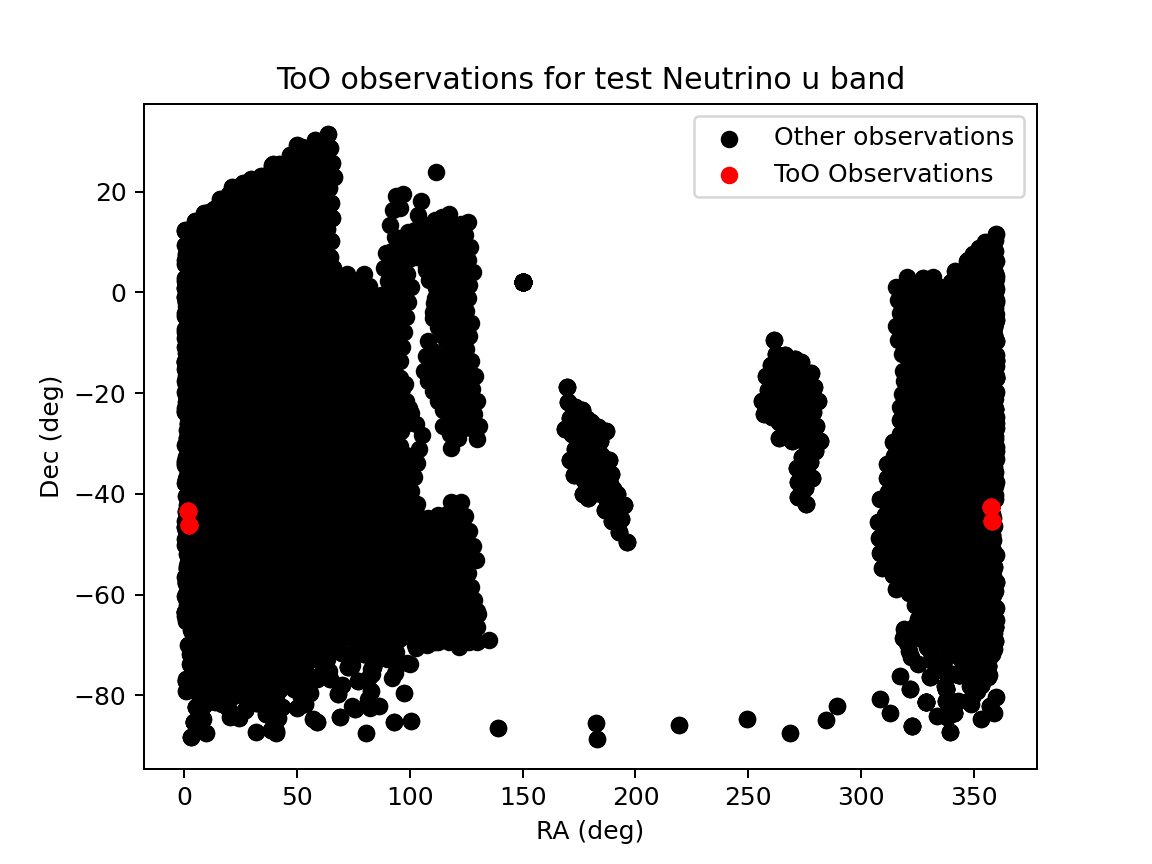
\includegraphics[width=\linewidth]{figures/validationTests/SVRequired/NeutrinoPosition.png}
    \caption{Results from a neutrino ToO visits over a 20 day LSST simulation}
    \label{fig:NeutrinoPositionResult}
\end{figure}

\begin{figure}
    \centering
    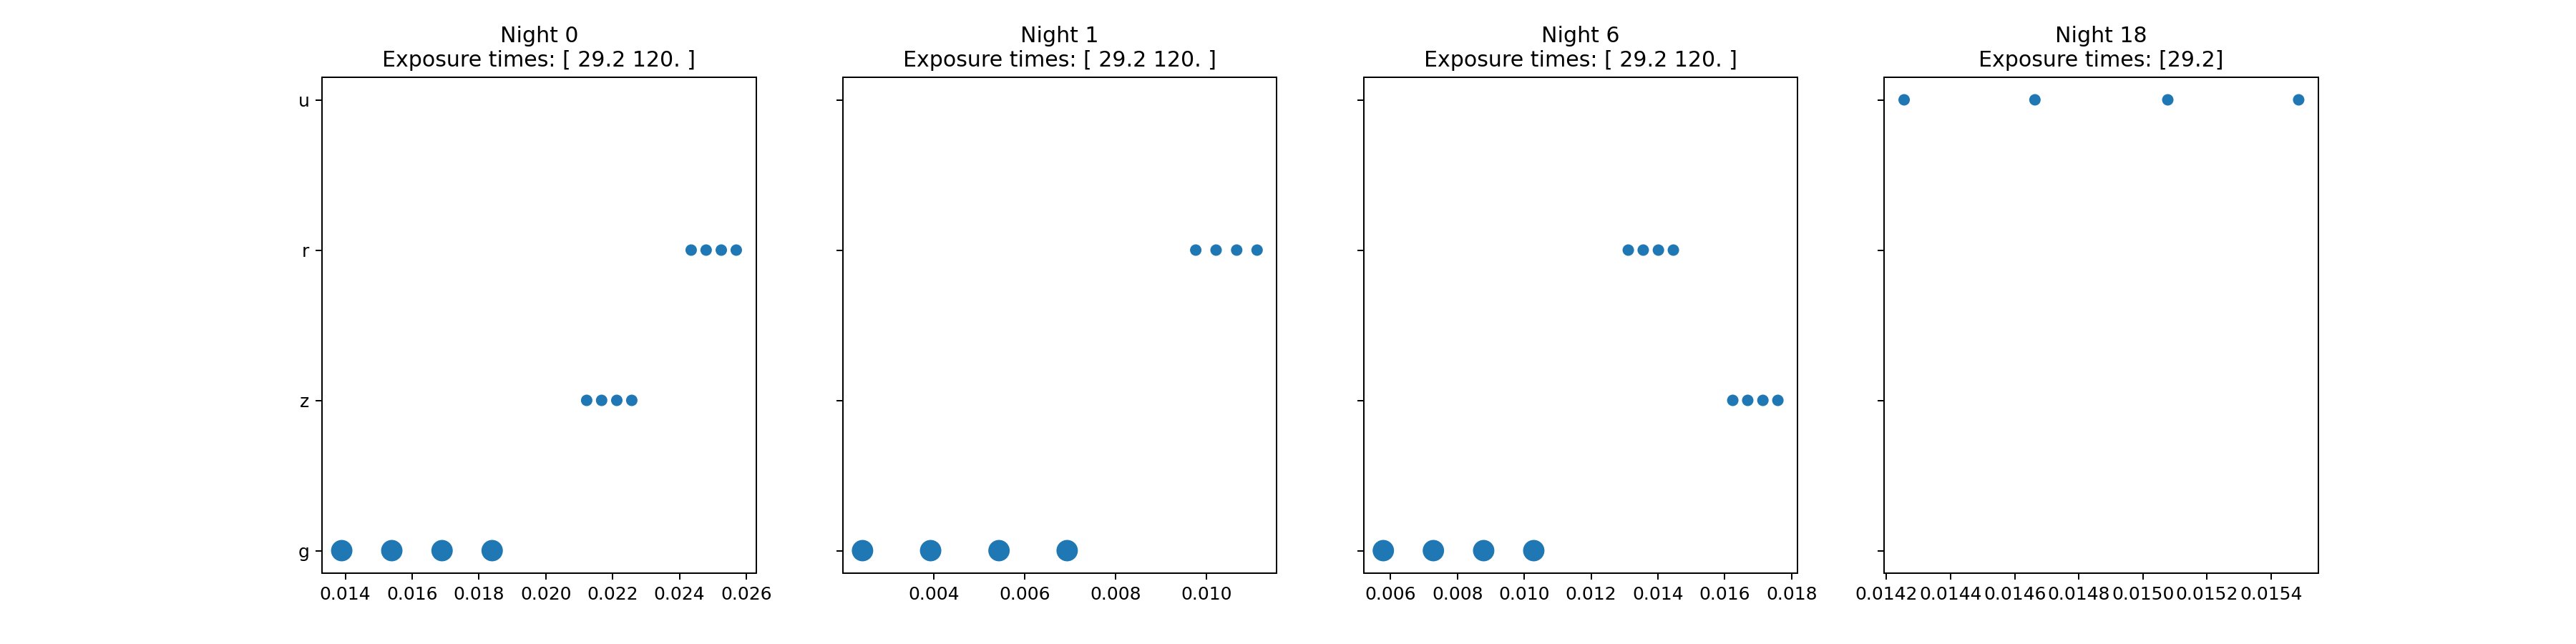
\includegraphics[width=\linewidth]{figures/validationTests/SVRequired/NeutrinoFilterPlot.png}
    \caption{Results from a neutrino ToO filter and visit distribution over a 20 day LSST simulation}
    \label{fig:NeutrinoFilterResult}
\end{figure}
\newpage


\subsection{Potentially hazardous asteroid}
\paragraph{Twilight}
\begin{table}[]
\centering
\begin{adjustbox}{max width=\textwidth}
\begin{tabular}{|l|l|l|l|l|l|l|l|}
\hline
Expected night & Resulting night & Expected visits & Resulting visits & Expected filters & Resulting filters & Expected exposure times & Resulting exposure times \\ \hline
0              & 0               & 1               & 1                & z                & z                 & 15                      & 15                       \\ \hline
\end{tabular}
\end{adjustbox}
\caption{Results from a potentially hazardous asteroid, twilight conditions ToO, filter and visit distribution over a 20 day LSST simulation}
\label{tab:PHATwiResult}
\end{table}

\begin{figure}
    \centering
    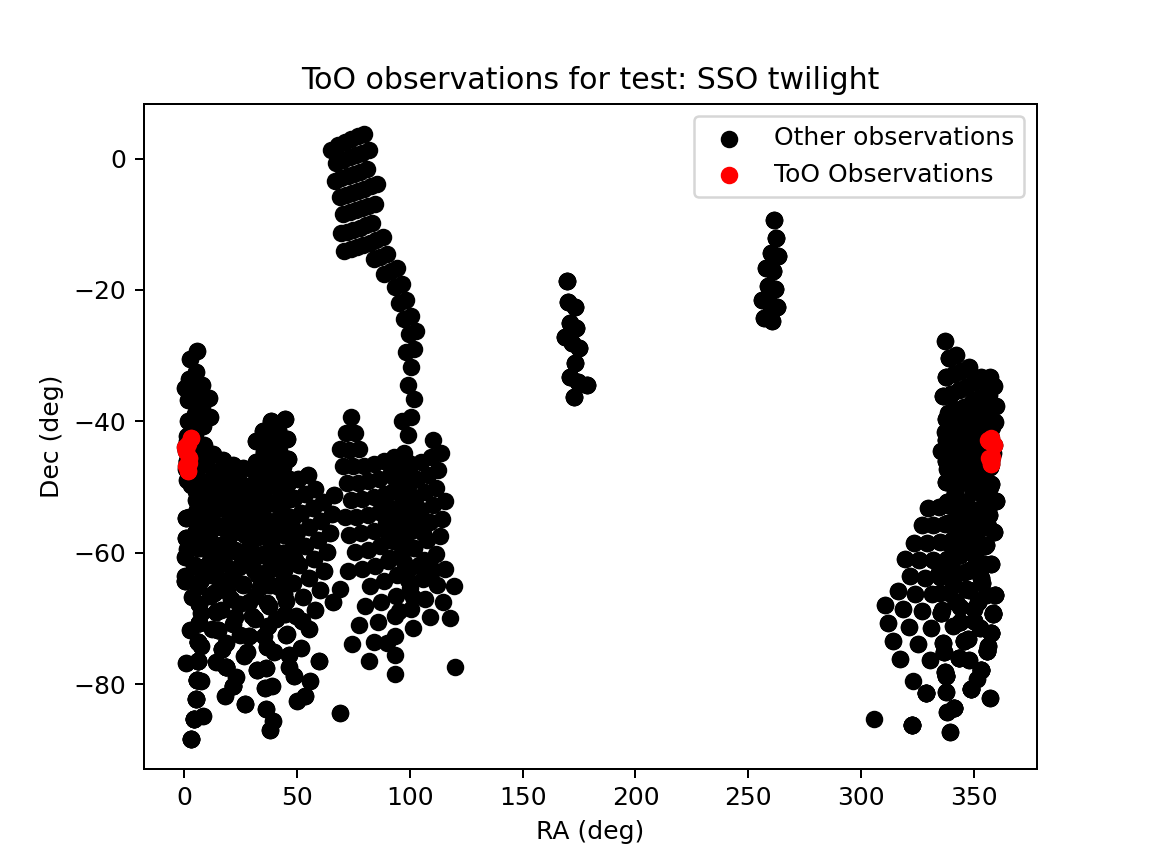
\includegraphics[width=\linewidth]{figures/validationTests/SVRequired/PHATwiPosition.png}
    \caption{Results from a potentially hazardous asteroid, twilight conditions ToO, visits over a 2 day LSST simulation}
    \label{fig:PHATwiPositionResult}
\end{figure}

\begin{figure}
    \centering
    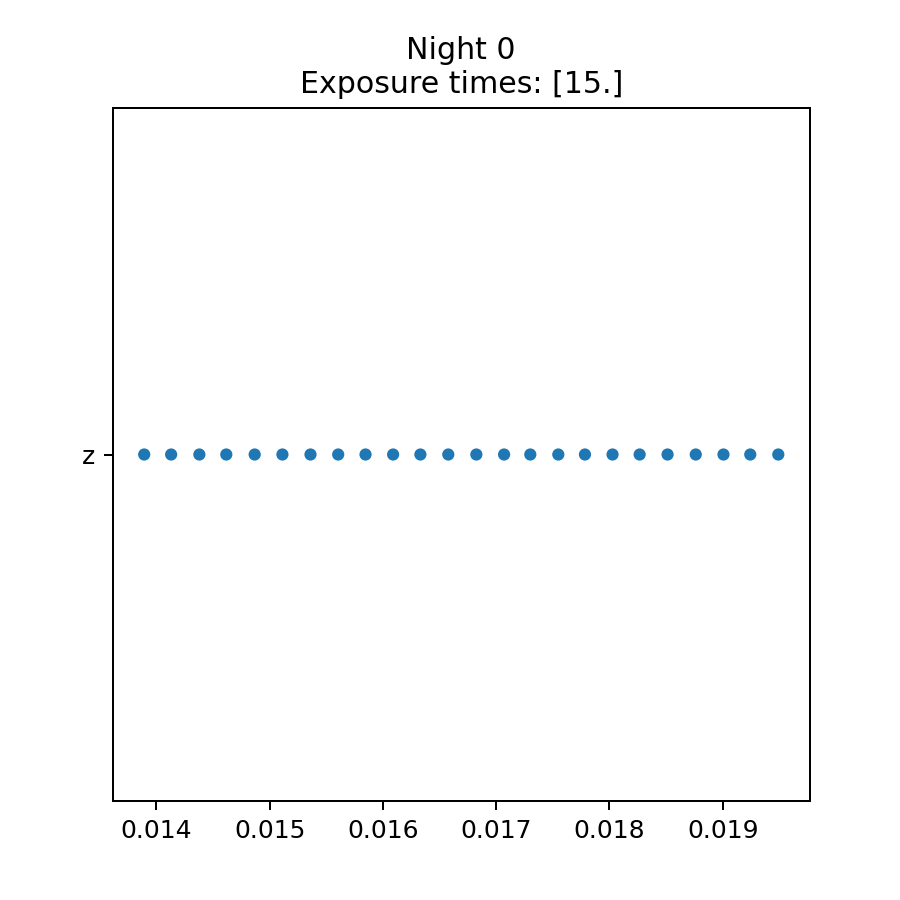
\includegraphics[width=\linewidth]{figures/validationTests/SVRequired/PHATwiFilterPlot.png}
    \caption{Results from a potentially hazardous asteroid, twilight conditions ToO, filter and visit distribution over a 2 day LSST simulation}
    \label{fig:PHATwiFilterResult}
\end{figure}
\newpage


\paragraph{Night}
\begin{table}[]
\centering
\begin{adjustbox}{max width=\textwidth}
\begin{tabular}{|l|l|l|l|l|l|l|l|}
\hline
Expected night & Resulting night & Expected visits & Resulting visits & Expected filters & Resulting filters & Expected exposure times & Resulting exposure times \\ \hline
0              & 0               & 1               & 1                & r                & r                 & 15                      & 15                       \\ \hline
\end{tabular}
\end{adjustbox}
\caption{Results from a potentially hazardous asteroid, night conditions ToO, filter and visit distribution over a 2 day LSST simulation}
\label{tab:PHANightResult}
\end{table}

\begin{figure}
    \centering
    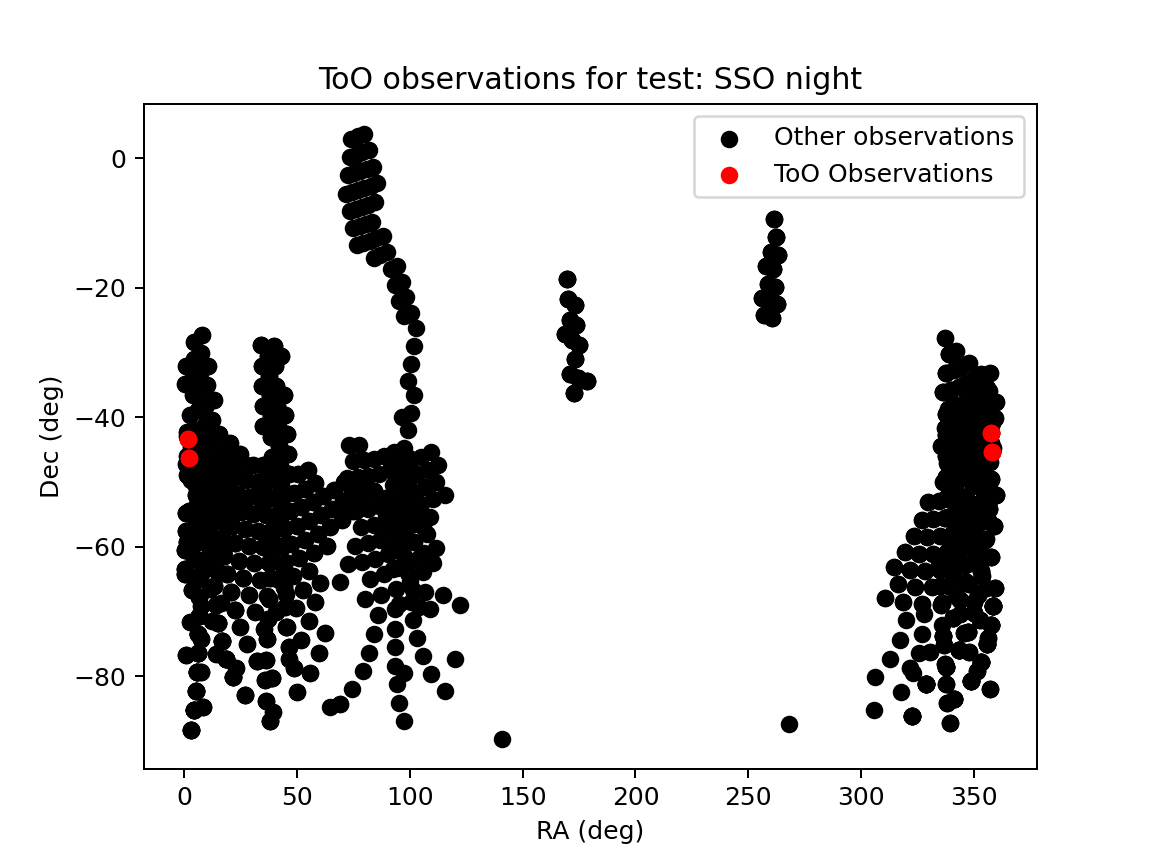
\includegraphics[width=\linewidth]{figures/validationTests/SVRequired/PHANightPosition.png}
    \caption{Results from a potentially hazardous asteroid, night conditions ToO, visits over a 2 day LSST simulation}
    \label{fig:PHANightPositionResult}
\end{figure}

\begin{figure}
    \centering
    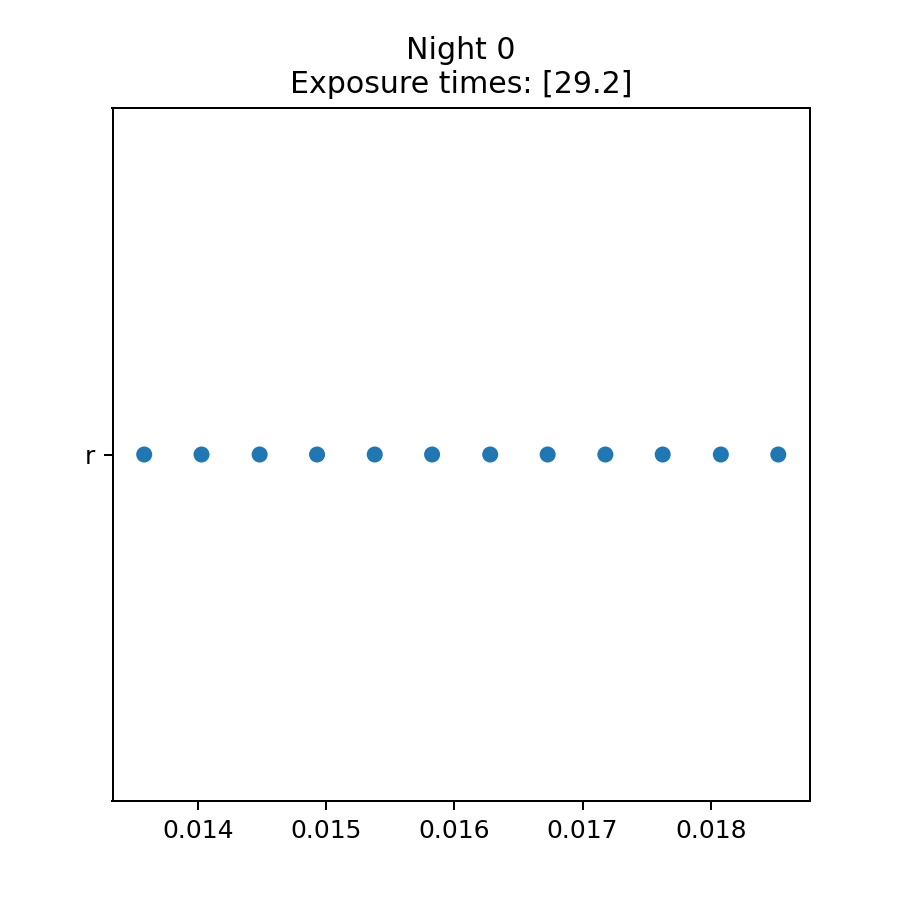
\includegraphics[width=\linewidth]{figures/validationTests/SVRequired/PHANightFilterPlot.png}
    \caption{Results from a potentially hazardous asteroid, night conditions ToO, filter and visit distribution over a 2 day LSST simulation}
    \label{fig:PHANightFilterResult}
\end{figure}
\newpage

\subsection{Additional ToO strategies}

\subsubsection{Galactic SN}

\begin{table}[]
\centering
\begin{adjustbox}{max width=\linewidth}
\begin{tabular}{|l|l|l|l|l|l|l|l|}
\hline
Expected night & Resulting night & Expected visits & Resulting visits & Expected filters & Resulting filters & Expected exposure times & Resulting exposure times \\ \hline
0              & 0               & 4               & 4                & i                & i                 & 1,15                    & 1,15                     \\ \hline
\end{tabular}
\end{adjustbox}
\caption{Results from a galactic SN ToO, filter and visit distribution over a 2 day LSST simulation}
\label{tab:GalacticSNResults}
\end{table}

\begin{figure}
    \centering
    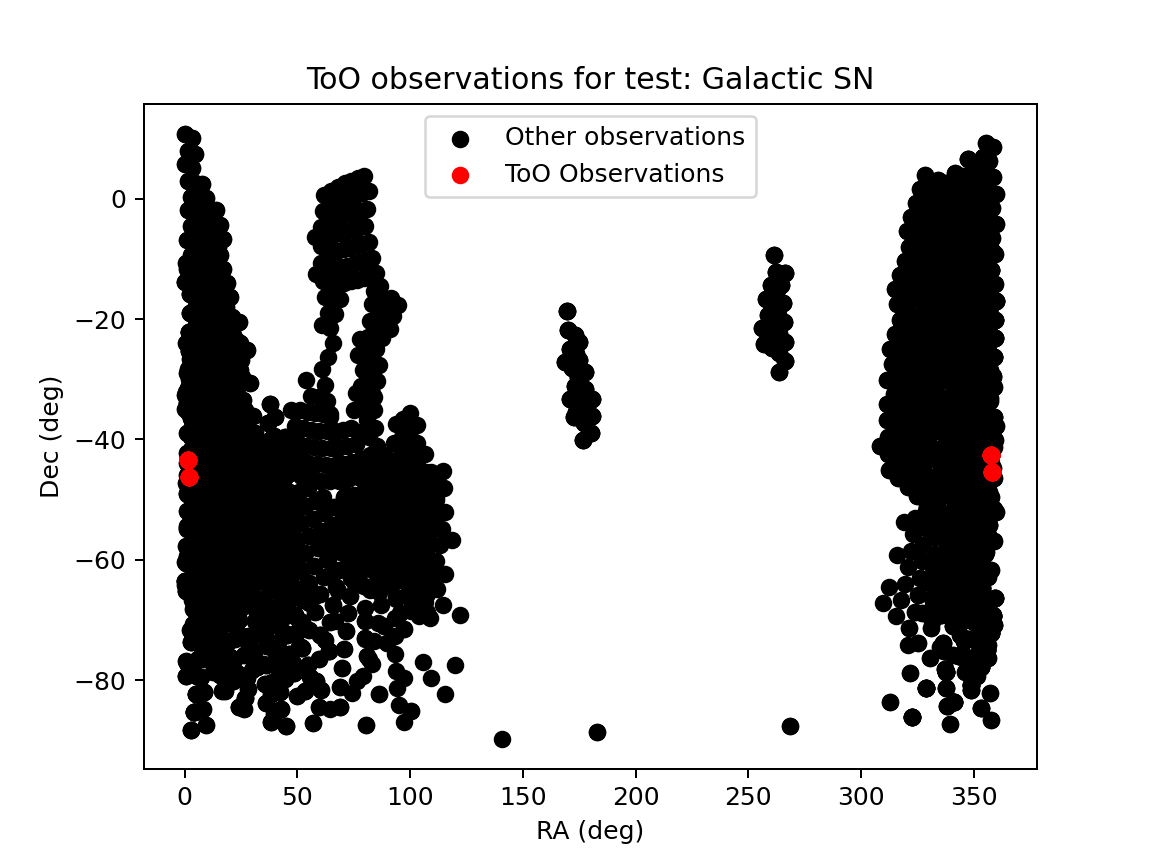
\includegraphics[width=\linewidth]{figures/validationTests/SVRequired/GalacticSNPosition.png}
    \caption{Results from a galactic SN ToO, visits over a 2 day LSST simulation}
    \label{fig:GalacticSNPositionResult}
\end{figure}

\begin{figure}
    \centering
    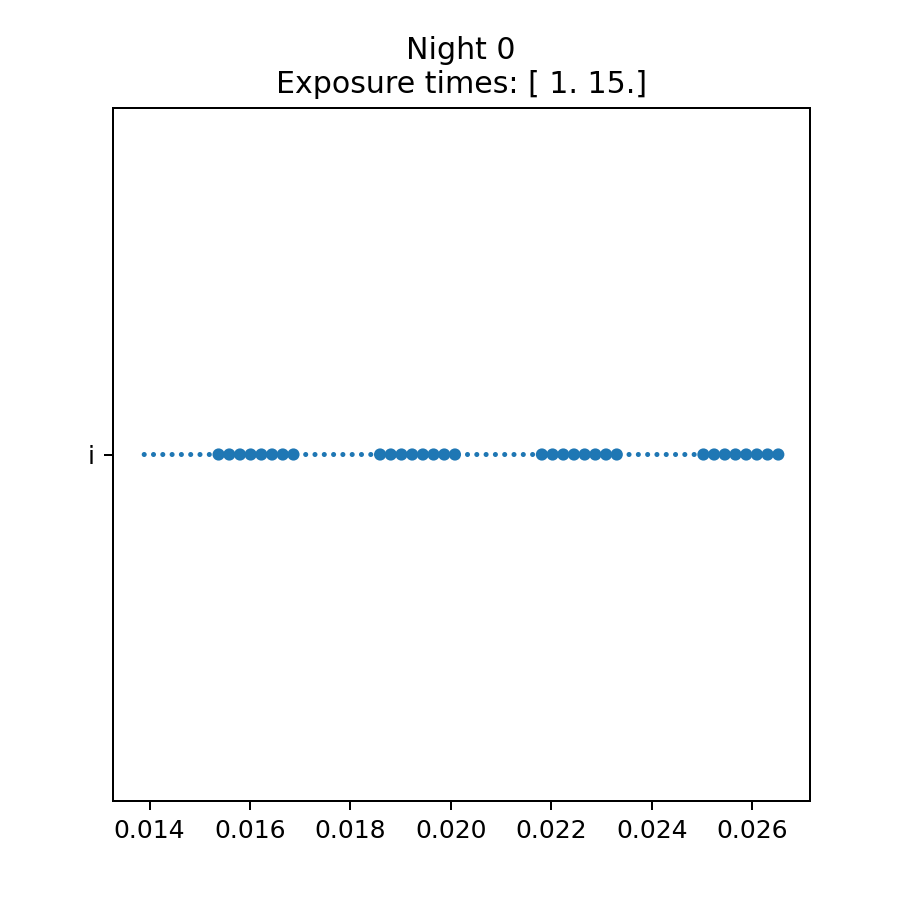
\includegraphics[width=\linewidth]{figures/validationTests/SVRequired/GalacticSNFilterPlot.png}
    \caption{Results from a galactic SN ToO, filter and visit distribution over a 2 day LSST simulation}
    \label{fig:GalacticSNFilterResult}
\end{figure}
\newpage
\subsubsection{Lensed BNS}

\paragraph{Large skymap}

\begin{table}[]
\centering
\begin{adjustbox}{max width=\linewidth}
\begin{tabular}{|l|l|l|l|l|l|l|l|}
\hline
Expected night & Resulting night & Expected visits & Resulting visits & Expected filters & Resulting filters & Expected exposure times & Resulting exposure times \\ \hline
0              & 0,1             & 1,3             & 1,3              & g,r              & g,r               & 30,30                   & 30,30                    \\ \hline
1              & 1,2,3           & 1,3             & 1,3              & g,r              & g,r               & 30,30                   & 30,30                    \\ \hline
2              & 3,4             & 1,3             & 1,3              & g,r              & g,r               & 30,30                   & 30,30                    \\ \hline
\end{tabular}
\end{adjustbox}
\caption{Results from a lensed BNS large skymap ToO, filter and visit distribution over a 10 day LSST simulation}
\label{tab:LensedBNSAResults}
\end{table}


\begin{figure}
    \centering
    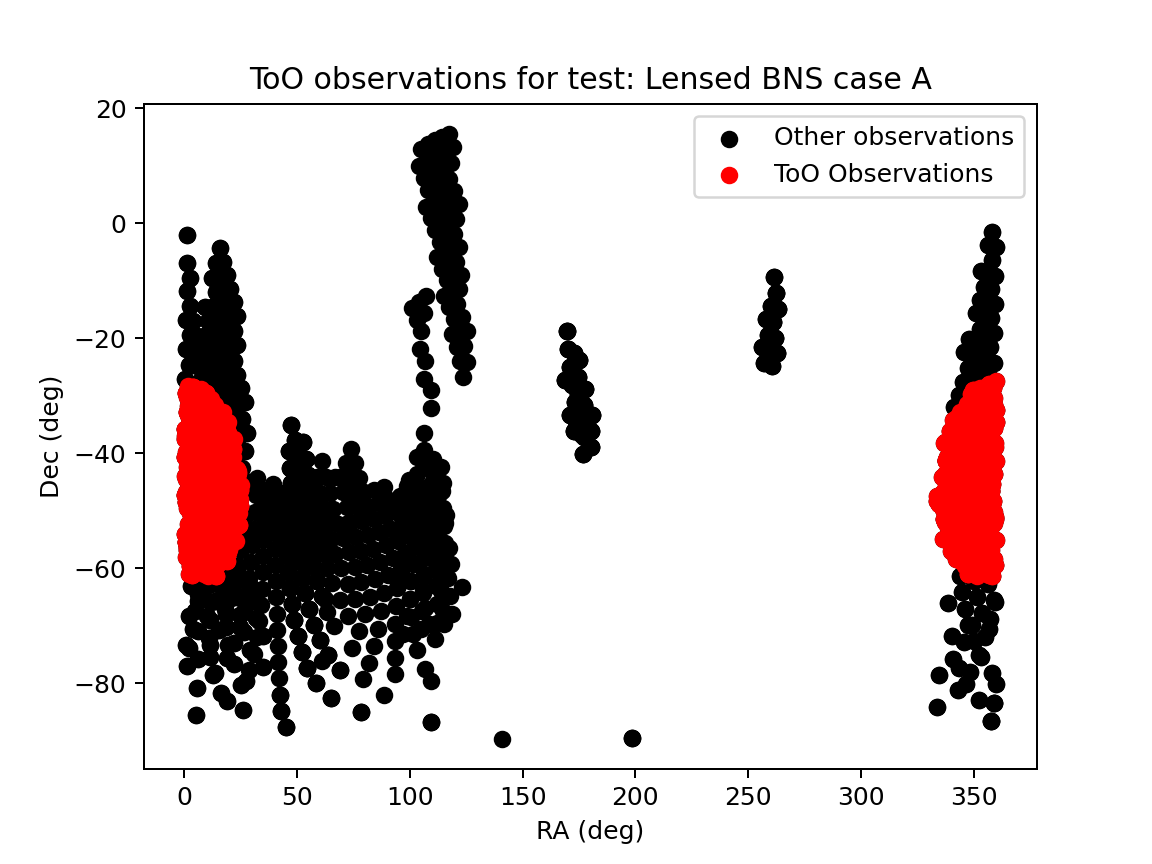
\includegraphics[width=\linewidth]{figures/validationTests/SVRequired/LensedBNSAPosition.png}
    \caption{Results from a lensed BNS large skymap ToO, visits over a 2 day LSST simulation}
    \label{fig:LensedBNSAPositionResult}
\end{figure}

\begin{figure}
    \centering
    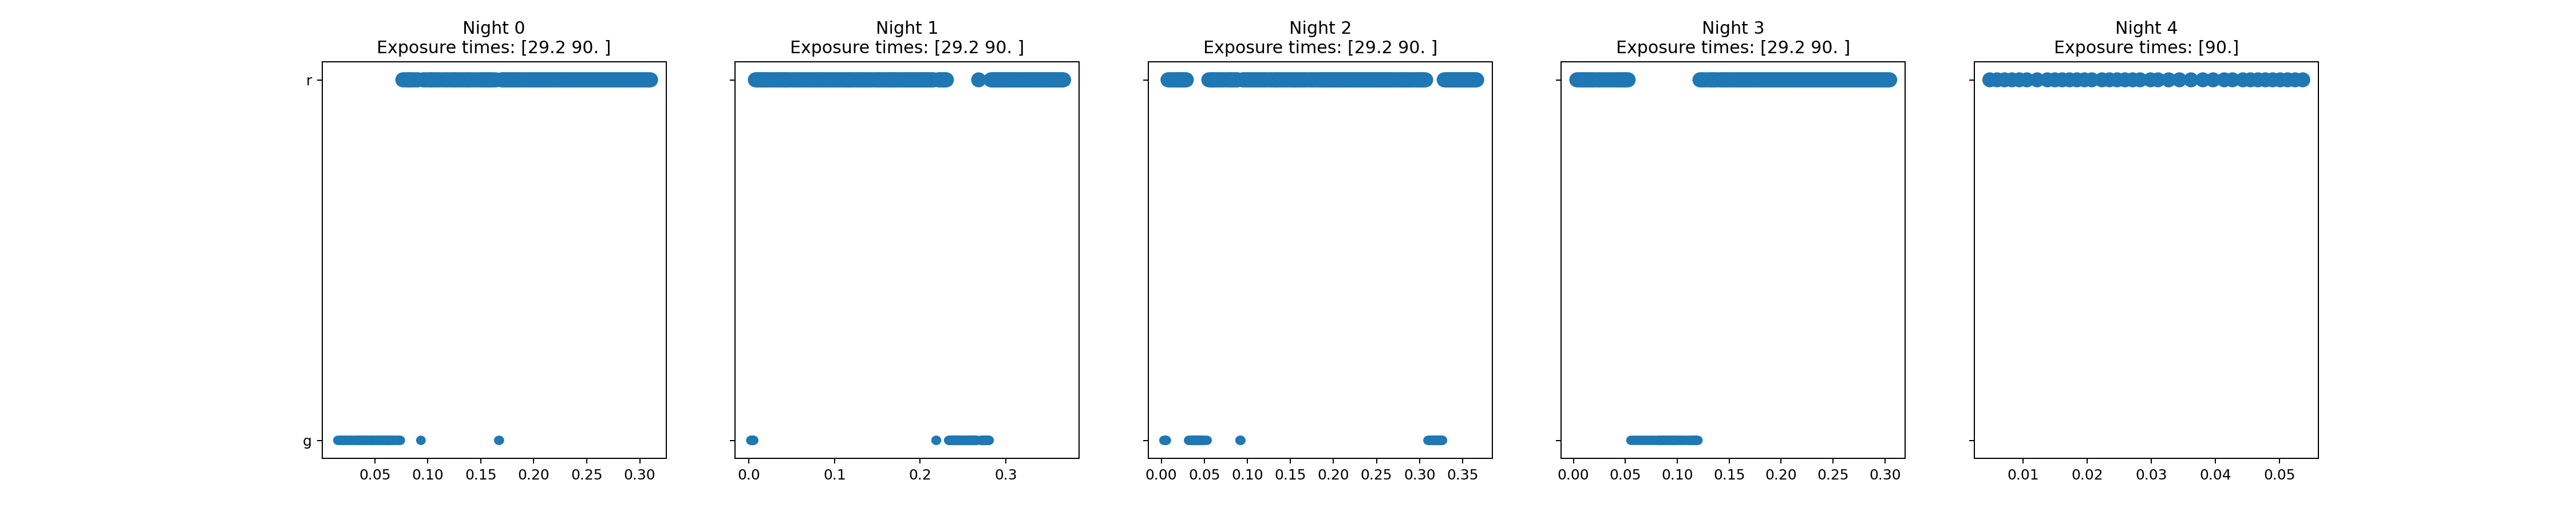
\includegraphics[width=\linewidth]{figures/validationTests/SVRequired/LensedBNSAFilterPlot.png}
    \caption{Results from a lensed BNS large skymap ToO, filter and visit distribution over a 2 day LSST simulation}
    \label{fig:LensedBNSAFilterResult}
\end{figure}
\newpage

\paragraph{Small skymap}

\begin{table}[]
\centering
\begin{adjustbox}{max width=\linewidth}
\begin{tabular}{|l|l|l|l|l|l|l|l|}
\hline
Expected night & Resulting night & Expected visits & Resulting visits & Expected filters & Resulting filters & Expected exposure times & Resulting exposure times \\ \hline
0              & 0,1             & 1               & 1                & g,r              & g,r               & 180                     & 180                      \\ \hline
1              & 1,2             & 1               & 1                & g,r              & g,r               & 180                     & 180                      \\ \hline
2              & 2,3             & 1               & 1                & g,r              & g,r               & 180                     & 180                      \\ \hline
\end{tabular}
\end{adjustbox}
\caption{Results from a lensed BNS large skymap ToO, filter and visit distribution over a 10 day LSST simulation}
\label{tab:LensedBNSBResults}
\end{table}

\begin{figure}
    \centering
    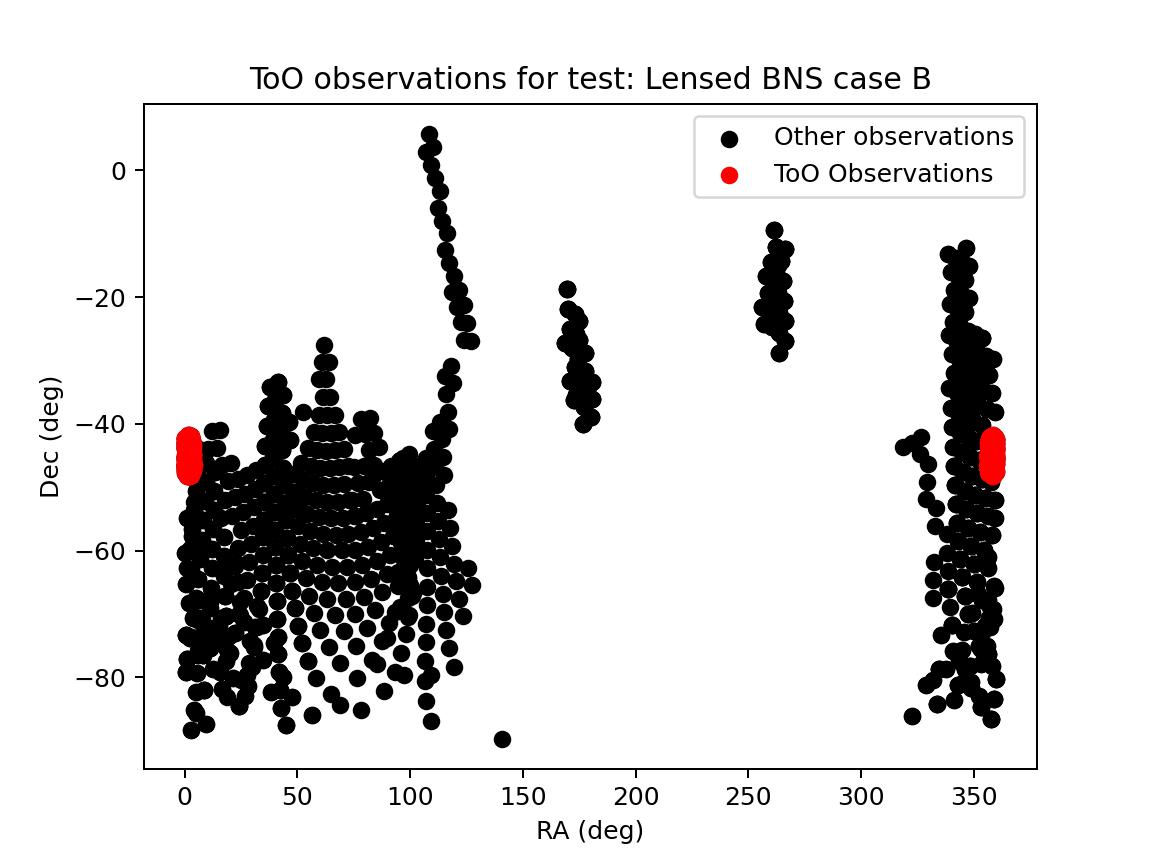
\includegraphics[width=\linewidth]{figures/validationTests/SVRequired/LensedBNSBPosition.png}
    \caption{Results from a lensed BNS large skymap ToO, visits over a 2 day LSST simulation}
    \label{fig:LensedBNSBPositionResult}
\end{figure}

\begin{figure}
    \centering
    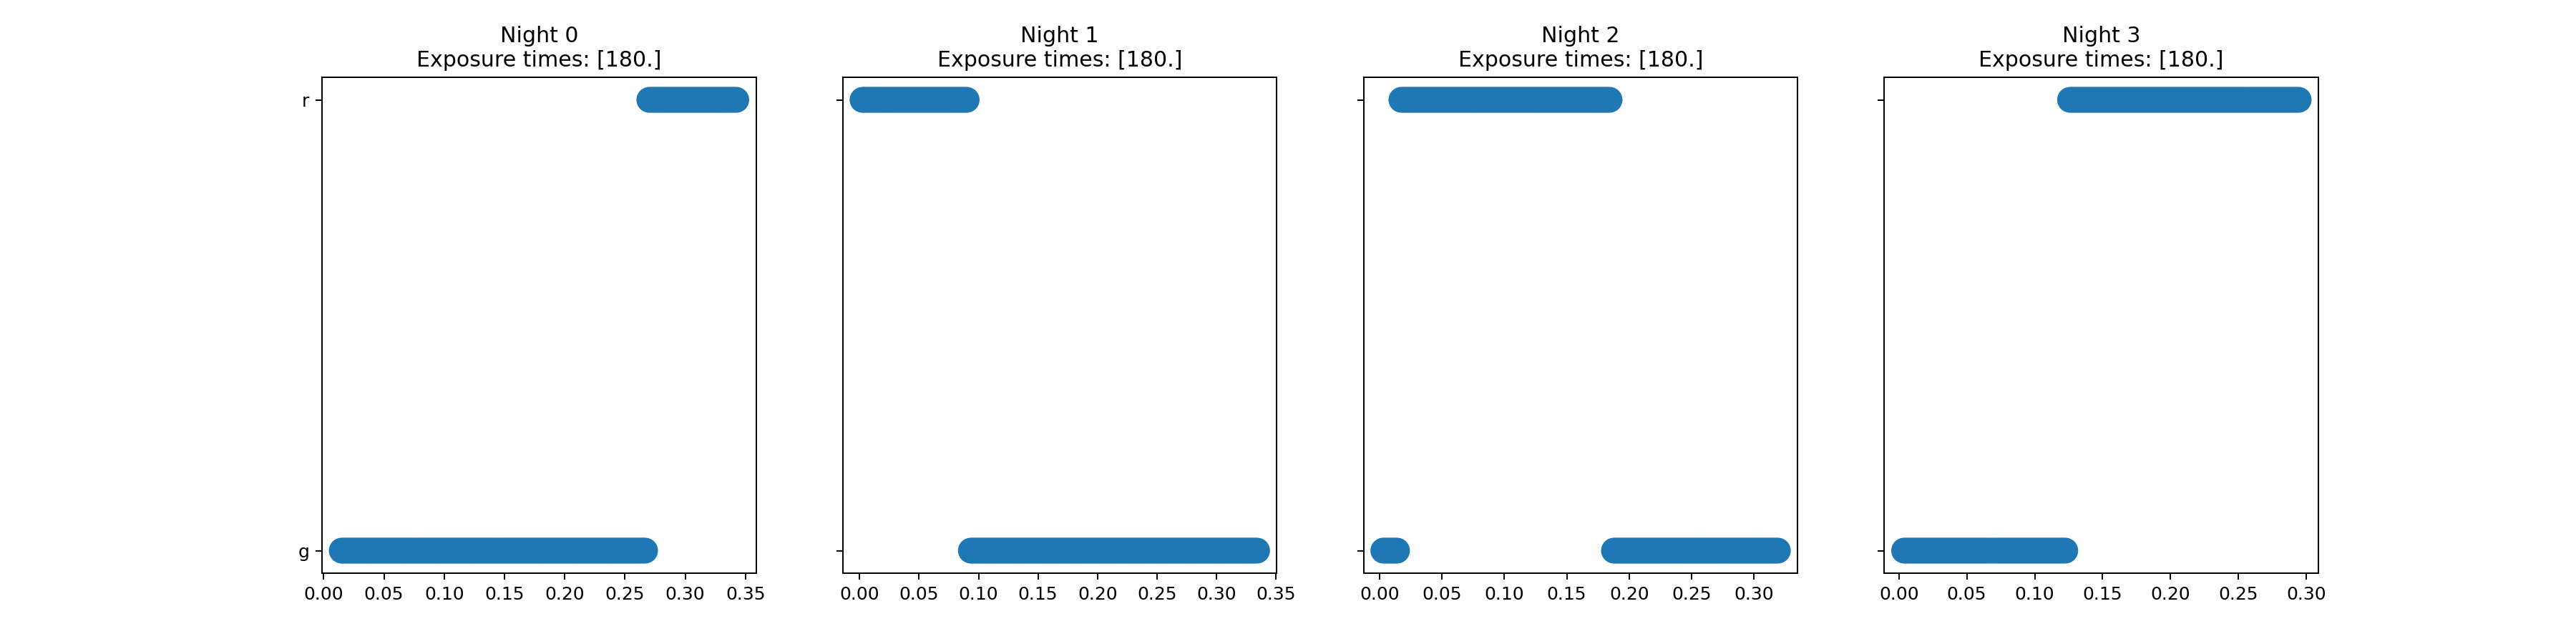
\includegraphics[width=\linewidth]{figures/validationTests/SVRequired/LensedBNSBFilterPlot.png}
    \caption{Results from a lensed BNS large skymap ToO, filter and visit distribution over a 2 day LSST simulation}
    \label{fig:LensedBNSBFilterResult}
\end{figure}
\newpage